\documentclass{article}

\usepackage{graphicx}
\usepackage{hyperref}
\usepackage{bm}
\usepackage{float}
\restylefloat{table}

\usepackage{listings}
\usepackage{color}
\usepackage{amsmath}

\usepackage[margin=1.25in]{geometry}

\definecolor{dkgreen}{rgb}{0,0.6,0}
\definecolor{gray}{rgb}{0.5,0.5,0.5}
\definecolor{mauve}{rgb}{0.86,0.27,0.22}

\lstset{frame=tb,
  language=python,
  aboveskip=3mm,
  belowskip=3mm,
  showstringspaces=false,
  columns=flexible,
  basicstyle={\small\ttfamily},
  numbers=none,
  numberstyle=\tiny\color{gray},
  keywordstyle=\color{blue},
  commentstyle=\color{dkgreen},
  stringstyle=\color{mauve},
  breaklines=true,
  breakatwhitespace=true,
  tabsize=3
}

%----------------------------------------------------------------------------------------
%	ASSIGNMENT INFORMATION
%----------------------------------------------------------------------------------------

\title{CS5200: Homework \#5} % Title of the assignment

\author{Matthew Whitesides\\ \texttt{mbwxd4@mst.edu}} % Author name and email address

\date{\today} % University, school and/or department name(s) and a date

%----------------------------------------------------------------------------------------

\begin{document}

  \maketitle % Print the title
 
  \begin{enumerate}
    \item \textbf{13.3-2 on p. 322.}
    
    So our goal is to insert and staisfy the cases:

    \begin{enumerate}
      \item All nodes are either red or black.
      \item Leaves are all black.
      \item Red nodes have black children.
      \item Equal number of black nodes in max paths.
      \item All internal nodes have two children – all leaves are NILs and are considered black.
    \end{enumerate}

    Our tree will be built like so {41, 38, 31, 12, 19, 8} (B = Black, R = Red):

    \begin{enumerate}
      \item Insert 41. Result: 41B.
      \item Insert 48. Result: 41B (left)$\rightarrow$ 38R.
      \item Insert 31. Result: 41B (left)$\rightarrow$ 38R (left)$\rightarrow$ 31R.
      \item Recolor 38R to 38B to staisfy case 3. Result: 41B (left)$\rightarrow$ 38B (left)$\rightarrow$ 31R.
      \item Recolor 41B to 41R to staisfy case 4. Result: 41R (left)$\rightarrow$ 38B (left)$\rightarrow$ 31R.
      \item Rotate to the right to balance the tree on 38. Result:\\
      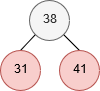
\includegraphics[scale=0.5]{1a.png}
      \item Insert 12 to the left of 31 to result in 12R.
      \item Recolor 31, 41 and 38 to black to keep case 3. Result:\\
      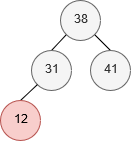
\includegraphics[scale=0.5]{1b.png}
      \item Insert 19R to the right of 12R. 
      \item Rotate left on 12R to put 19R above 12R.
      \item Rotate right on 19R to balance and put 12R and 31 below 19R.
      \item Recolor 19R to black to staisfy caes 4. Result:\\
      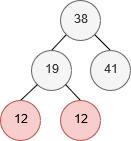
\includegraphics[scale=0.5]{1c.png}
      \item Insert 8R to the left of 12R.
      \item Recolor 12R and 31R to black, and recolor 19B to red to satisfy case 4. Final Result:\\
      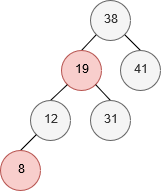
\includegraphics[scale=0.5]{1d.png}

    \end{enumerate}

    \item \textbf{13.4-3 on p. 330.}
    
    Remove {8, 12, 19, 31, 38, 41}:

    \begin{enumerate}
      \item Remove 8:\\
      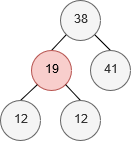
\includegraphics[scale=0.5]{2a.png}
      \item Remove 12.
      \item Recolor 19 to black.\\
      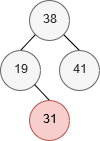
\includegraphics[scale=0.5]{2b.png}
      \item Rotate 19 right to put 31 above 19.
      \item Remove 19.\\
      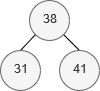
\includegraphics[scale=0.5]{2c.png}
      \item Recolor 31 and 41 to red.
      \item Remove 31.\\
      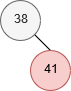
\includegraphics[scale=0.5]{2d.png}
      \item Remove 41.\\
      
\includegraphics[scale=0.5]{2e.png}
      \item Finally remove 38.
    \end{enumerate}

    \item \textbf{15.2-2 on p. 378. Implement your algorithm.}
    
    TODO!!!!!

    \item \textbf{15.4-1 on p. 396.}
    
    The longest common subsequence of $\left\{ 1, 0, 0, 1, 0, 1, 0, 1 \right\}$ and $\left\{ 0, 1, 0, 1, 1, 0, 1, 1, 0 \right\}$ would be \bm{$\left\{ 1, 0, 0, 1, 1, 0 \right\}$}.
    
    Note however there could be more than one of this length.

    You could find this using an iterative substring algorithm like so:

    \begin{lstlisting}
      def lcs(s1, s2):
      table = [["" for x in range(len(s2))] for x in range(len(s1))]
      for i in range(len(s1)):
          for j in range(len(s2)):
              if s1[i] == s2[j]:
                  if i == 0 or j == 0:
                      table[i][j] = s1[i]
                  else:
                      table[i][j] = table[i-1][j-1] + s1[i]
              else:
                  table[i][j] = max(table[i-1][j], table[i][j-1], key=len)
      return table[-1][-1]

      print(lcs("10010101", "010110110"));

      #Output: 100110
    \end{lstlisting}

    \item \textbf{15.4-5 on p. 397. Just describe the algorithm.}
    
    To find the longest monotonically increasing sub-sequence of a sequence of n numbers, in $O(n^2)$ time would go something like so:

    \begin{enumerate}
      \item Let $S\;=\;a\;sequence\;of\;n\;numbers$.
      \item Let $LMIS\;of\;S\;=\;Longest\;Monotonically\;Increasing\;Sub Sequence\;of\;S$.
      \item For $i\;in\;range(n)$ let Monotonically increasing sub sequence $mis(i)$ be the length of the longest $mis(i)$ for $sequence s\;in\;s_1, s_2, ... s_i$.
      \item Thus we seek the max length of the sequence $mis(i) \in i \in range(n)$.
      \item We'll want to find the LMIS of each MIS(i) and fill in a table of each value, then find the longest value in the table to find the LMIS(n).
      \item To find the MIS(i) recursively go trough to find the $LMIS(s_{i - 1})$ until you hit the base case of i = 1 which the LMIS of a sequence of one is the element itself. 
      \item Then for each other case check (lets call the recursive call iteration $j$) if $j \leq i -1$ you keep going otherwise return to finish the recursion. 
      \item Once you have finished for each sub sequence $s$ in $S$ you scan the table for the longest value.
      \item The recusive part to fill the table would take $O(n^2)$ time and the part to find the max value in the table would take $O(n)$ time giving a total of $O(n^2)$.
    \end{enumerate}

    \item \textbf{16.1-3 on p. 422.}
    
    \begin{itemize}
      \item Show that the approach of selecting the activity of least duration from among those that are compatible with previously selected activities does not work.
      \begin{itemize}
        \item Say we have the following start and finsih times.
          \begin{table}[H]
            \centering
            \begin{tabular}{|l|lll}
            \hline
            $i$   & \multicolumn{1}{l|}{1} & \multicolumn{1}{l|}{2} & \multicolumn{1}{l|}{3} \\ \hline
            $s_i$ & 0                      & 4                      & 6                      \\ \cline{1-1}
            $f_i$ & 5                      & 7                      & 10                     \\ \cline{1-1}
            \end{tabular}
          \end{table}
        \item Using greedy we'd pick 4 - 7 first as it's the shortest length however since it overlaps with both column 1 and 3 we'd eliminate both those, however they don't overlap eachother so we could have had two periods instead of just the one.
      \end{itemize}
      \item Do the same for the approaches of always selecting the compatible activity that overlaps the fewest other remaining activities.
      \begin{itemize}
        \item Say we have the following table.
        
        \begin{table}[H]
          \centering
          \begin{tabular}{|l|lllllllllll}
          \hline
          $i$   & \multicolumn{1}{l|}{1} & \multicolumn{1}{l|}{2} & \multicolumn{1}{l|}{3} & \multicolumn{1}{l|}{4} & \multicolumn{1}{l|}{5} & \multicolumn{1}{l|}{6} & \multicolumn{1}{l|}{7} & \multicolumn{1}{l|}{8} & \multicolumn{1}{l|}{9} & \multicolumn{1}{l|}{10} & \multicolumn{1}{l|}{11} \\ \hline
          $s_i$ & 0                      & 1                      & 1                      & 1                      & 3                      & 5                      & 7                      & 9                      & 9                      & 9                       & 11                      \\ \cline{1-1}
          $f_i$ & 2                      & 4                      & 4                      & 4                      & 6                      & 8                      & 10                     & 12                     & 12                     & 12                      & 13                      \\ \cline{1-1}
          \end{tabular}
        \end{table}

        \item Essentailly this is the easist thing I could think of you have everything but the middle column with three conflicts where i=6 has two. That would give you columns 6,1,8 using greedy lest conflicts however a more optimal solution would be columns 1,5,7,11.
      \end{itemize}
      \item And for always selecting the compatible remaining activity with the earliest start time.
      \begin{itemize}
        \item Say we have the following table.
        \begin{table}[H]
          \centering
          \begin{tabular}{|l|lll}
          \hline
          $i$   & \multicolumn{1}{l|}{1} & \multicolumn{1}{l|}{2} & \multicolumn{1}{l|}{3} \\ \hline
          $s_i$ & 0                      & 1                      & 6                      \\ \cline{1-1}
          $f_i$ & 7                      & 5                      & 10                     \\ \cline{1-1}
          \end{tabular}
        \end{table}
        \item Here we'd instantly pick column 1 and only have one period insead of being able to fit in two if we went with columns 2 \& 3.
      \end{itemize}
    \end{itemize}

    \item \textbf{16.2-5 on p. 428. Just describe the algorithm.}
    
    Given we're talking about greedy algorithms I figure we'll try to set up oneo f those to get an optimal smallest set of closed intervals that contains all the given points.

    \begin{enumerate}
      \item First sort the points by value so they are monotonically increasing in order $x_1, x_2, x_n$.
      \item 
    \end{enumerate}

    \item \textbf{16.3-3 on p. 436.}
    \item \textbf{17.4-3 on p. 471.}
    \item \textbf{18.2-1 on p. 497.}
    \item \textbf{18.3-1 on p. 350.}
    \item \textbf{19.2-1 on p. 518.}
    \item \textbf{19.4-1 on p. 526.}
    \item \textbf{21.3-2 on p. 572. Implement your algorithm.}
  \end{enumerate}

\end{document}
